Oblicz wartość średnią sygnału $f(t)=\mathbf{1}(t)\cdot e^{-a\cdot t}\cdot sin\left(\frac{2\pi}{T}\cdot t \right )$ przedstawionego na rysunku 

\begin{figure}[H]
\centering
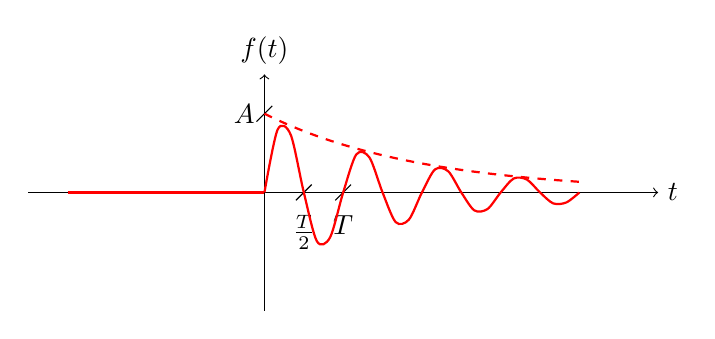
\begin{tikzpicture}
  %\draw (0,0) circle (1in);
  \draw[->] (-3.0,+0.0) -- (+5.0,+0.0) node[right] {$t$};
  \draw[->] (+0.0,-1.5) -- (+0.0,+1.5) node[above] {$f(t)$};
  \draw[-,red, thick] (-2.5,+0.0) -- (+0.0,+0.0);
  %\draw[-] (-1.0-0.1,-0.1)--(-1.0+0.1,0.1) node[midway, below, outer sep=10pt,align=center] {$-\frac{T}{2}$};
  \draw[-] (+0.5-0.1,-0.1)--(+0.5+0.1,0.1) node[midway, below, outer sep=5pt] {$\frac{T}{2}$};
  \draw[-] (+1.0-0.1,-0.1)--(+1.0+0.1,0.1) node[midway, below, outer sep=5pt] {$T$};
  \draw[-] (-0.1,1.0-0.1)--(+0.1,1.0+0.1) node[midway, left] {$A$};
  
  \draw[scale=1.0,domain=0:4.0,smooth,variable=\x,red,thick] plot ({\x},{exp(-0.5*\x)*sin(\x*180.0/3.141592*2*3.141592/1.0)});
  
  \draw[scale=1.0,domain=0:4.0,smooth,variable=\x,red,thick,dashed] plot ({\x},{exp(-0.5*\x)});
\end{tikzpicture}
\end{figure}

Wartość średnią sygnału wyznaczamy z wzoru

\begin{equation}
\bar{f}=\lim_{\tau \rightarrow \infty }\frac{1}{\tau}\int_{-\frac{\tau}{2}}^{\frac{\tau}{2}}f(t) \cdot dt
\end{equation}

Podstawiamy do wzoru wzór naszej funkcji

%\begin{equation}
%\begin{aligned}
\begin{align*}
\bar{f} &=\lim_{\tau \rightarrow \infty }\frac{1}{\tau}\int_{-\frac{\tau}{2}}^{\frac{\tau}{2}}f(t) \cdot dt\\
 &=\lim_{\tau \rightarrow \infty }\frac{1}{\tau}\int_{-\frac{\tau}{2}}^{\frac{\tau}{2}} \mathbf{1}(t)\cdot e^{-a\cdot t}\cdot sin\left(\frac{2\pi}{T}\cdot t \right) \cdot dt\\
 &=\lim_{\tau \rightarrow \infty }\frac{1}{\tau}\left(
 \int_{-\frac{\tau}{2}}^{0} 0 \cdot e^{-a\cdot t}\cdot sin\left(\frac{2\pi}{T}\cdot t \right) \cdot dt +
 \int_{0}^{\frac{\tau}{2}} 1 \cdot e^{-a\cdot t}\cdot sin\left(\frac{2\pi}{T}\cdot t \right) \cdot dt \right)\\
 &=\lim_{\tau \rightarrow \infty }\frac{1}{\tau}\left(
 \int_{-\frac{\tau}{2}}^{0} 0 \cdot dt +
 \int_{0}^{\frac{\tau}{2}} e^{-a\cdot t}\cdot sin\left(\frac{2\pi}{T}\cdot t \right) \cdot dt \right)\\
 &=\lim_{\tau \rightarrow \infty }\frac{1}{\tau}\left(
 0 +
 \int_{0}^{\frac{\tau}{2}} e^{-a\cdot t}\cdot sin\left(\frac{2\pi}{T}\cdot t \right) \cdot dt \right)\\
 &=\lim_{\tau \rightarrow \infty }\frac{1}{\tau}\left(
 \int_{0}^{\frac{\tau}{2}} e^{-a\cdot t}\cdot sin\left(\frac{2\pi}{T}\cdot t \right) \cdot dt \right)\\
 &=\begin{Bmatrix*}[l]
 u=sin(\frac{2\pi}{T}\cdot t) & dv = e^{-a \cdot t}\cdot dt\\ 
 du=\frac{2\pi}{T} \cdot cos(\frac{2\pi}{T}\cdot t)\cdot dt & v=-\frac{1}{a}\cdot e^{-a\cdot t}
 \end{Bmatrix*}\\
 &=\lim_{\tau \rightarrow \infty }\frac{1}{\tau}\left(
 \left. -\frac{1}{a}\cdot e^{-a\cdot t} \cdot sin \left(\frac{2\pi}{T}\cdot t\right) \right|_{0}^{\frac{\tau}{2}}
 -\int_{0}^{\frac{\tau}{2}} -\frac{1}{a}\cdot e^{-a\cdot t} \cdot \frac{2\pi}{T} \cdot cos\left(\frac{2\pi}{T}\cdot t\right)\cdot dt
 \right)\\
 &=\lim_{\tau \rightarrow \infty }\frac{1}{\tau}\left(
 \left( -\frac{1}{a}\cdot e^{-a\cdot \frac{\tau}{2}} \cdot sin \left(\frac{2\pi}{T}\cdot \frac{\tau}{2}\right) + \frac{1}{a}\cdot e^{-a\cdot 0} \cdot sin \left(\frac{2\pi}{T}\cdot 0\right) \right)\right.\\
 &\left.+\frac{1}{a} \cdot \frac{2\pi}{T} \cdot \int_{0}^{\frac{\tau}{2}} \cdot e^{-a\cdot t} \cdot cos\left(\frac{2\pi}{T}\cdot t\right)\cdot dt \right)\\
 &=\begin{Bmatrix*}[l]
 u=cos(\frac{2\pi}{T}\cdot t) & dv = e^{-a \cdot t}\cdot dt\\ 
 du=-\frac{2\pi}{T} \cdot sin(\frac{2\pi}{T}\cdot t)\cdot dt & v=-\frac{1}{a}\cdot e^{-a\cdot t}
 \end{Bmatrix*}\\
 &=\lim_{\tau \rightarrow \infty }\frac{1}{\tau}\left(
 \left( -\frac{1}{a}\cdot e^{-a\cdot \frac{\tau}{2}} \cdot sin \left(\frac{2\pi}{T}\cdot \frac{\tau}{2}\right) + \frac{1}{a}\cdot e^{-a\cdot 0} \cdot sin \left(\frac{2\pi}{T}\cdot 0\right) \right)\right.\\
 &\left.+\frac{1}{a} \cdot \frac{2\pi}{T} \cdot 
 \left(
 \left. -\frac{1}{a}\cdot e^{-a\cdot t} \cdot cos \left(\frac{2\pi}{T}\cdot t\right) \right|_{0}^{\frac{\tau}{2}}
 -\int_{0}^{\frac{\tau}{2}} -\frac{1}{a}\cdot e^{-a\cdot t} \cdot \frac{2\pi}{T} \cdot sin\left(\frac{2\pi}{T}\cdot t\right)\cdot dt
 \right)
 \right)\\
 &=\lim_{\tau \rightarrow \infty }\frac{1}{\tau}\left(
 \left( -\frac{1}{a}\cdot e^{-a\cdot \frac{\tau}{2}} \cdot sin \left(\frac{2\pi}{T}\cdot \frac{\tau}{2}\right) + \frac{1}{a}\cdot 1 \cdot 0 \right)\right.\\
 &\left.+\frac{1}{a} \cdot \frac{2\pi}{T} \cdot 
 \left(
 \left( -\frac{1}{a}\cdot e^{-a\cdot \frac{\tau}{2}} \cdot cos \left(\frac{2\pi}{T}\cdot \frac{\tau}{2}\right) + \frac{1}{a}\cdot e^{-a\cdot 0} \cdot cos \left(\frac{2\pi}{T}\cdot 0\right) \right)
 \right.\right. \\
 &\left.\left.+\frac{1}{a}\cdot \frac{2\pi}{T} \cdot \int_{0}^{\frac{\tau}{2}} e^{-a\cdot t} \cdot  sin\left(\frac{2\pi}{T}\cdot t\right)\cdot dt
 \right)
 \right)\\
 &=\lim_{\tau \rightarrow \infty }\frac{1}{\tau}\left(
 \left( -\frac{1}{a}\cdot e^{-a\cdot \frac{\tau}{2}} \cdot sin \left(\frac{2\pi}{T}\cdot \frac{\tau}{2}\right) + 0 \right)\right.\\
 &\left.+\frac{1}{a} \cdot \frac{2\pi}{T} \cdot 
 \left(
 \left( -\frac{1}{a}\cdot e^{-a\cdot \frac{\tau}{2}} \cdot cos \left(\frac{2\pi}{T}\cdot \frac{\tau}{2}\right) + \frac{1}{a}\cdot 1 \cdot 1 \right)
 \right.\right. \\
 &\left.\left.+\frac{1}{a}\cdot \frac{2\pi}{T} \cdot \int_{0}^{\frac{\tau}{2}} e^{-a\cdot t} \cdot  sin\left(\frac{2\pi}{T}\cdot t\right)\cdot dt
 \right)
 \right)\\
 &=\lim_{\tau \rightarrow \infty }\frac{1}{\tau}\left(
 -\frac{1}{a}\cdot e^{-a\cdot \frac{\tau}{2}} \cdot sin \left(\frac{2\pi}{T}\cdot \frac{\tau}{2}\right)\right.\\
 &\left.-\frac{1}{a^2} \cdot \frac{T}{2\pi} \cdot 
 e^{-a\cdot \frac{\tau}{2}} \cdot cos \left(\frac{2\pi}{T}\cdot \frac{\tau}{2}\right) + \frac{1}{a^2}\cdot \frac{T}{2\pi}
 \right. \\
 &\left.+\frac{1}{a^2}\cdot \frac{T^2}{4\pi^2} \cdot \int_{0}^{\frac{\tau}{2}} e^{-a\cdot t} \cdot  sin\left(\frac{2\pi}{T}\cdot t\right)\cdot dt
 \right)\\
 &=\begin{Bmatrix*}[l]
 -\frac{1}{a}\cdot e^{-a\cdot \frac{\tau}{2}} \cdot sin \left(\frac{2\pi}{T}\cdot \frac{\tau}{2}\right)\\
 -\frac{1}{a^2} \cdot \frac{T}{2\pi} \cdot 
 e^{-a\cdot \frac{\tau}{2}} \cdot cos \left(\frac{2\pi}{T}\cdot \frac{\tau}{2}\right) + \frac{1}{a^2}\cdot \frac{T}{2\pi}
  \\
 +\frac{1}{a^2}\cdot \frac{T^2}{4\pi^2} \cdot \int_{0}^{\frac{\tau}{2}} e^{-a\cdot t} \cdot  sin\left(\frac{2\pi}{T}\cdot t\right)\cdot dt = \int_{0}^{\frac{\tau}{2}} e^{-a\cdot t} \cdot  sin\left(\frac{2\pi}{T}\cdot t\right)\cdot dt
 \end{Bmatrix*}\\
 &=\begin{Bmatrix*}[l]
 -\frac{1}{a}\cdot e^{-a\cdot \frac{\tau}{2}} \cdot sin \left(\frac{2\pi}{T}\cdot \frac{\tau}{2}\right)
 -\frac{1}{a^2} \cdot \frac{T}{2\pi} \cdot 
 e^{-a\cdot \frac{\tau}{2}} \cdot cos \left(\frac{2\pi}{T}\cdot \frac{\tau}{2}\right) + \frac{1}{a^2}\cdot \frac{T}{2\pi}
  \\
 = \int_{0}^{\frac{\tau}{2}} e^{-a\cdot t} \cdot  sin\left(\frac{2\pi}{T}\cdot t\right)\cdot dt - \frac{1}{a^2}\cdot \frac{T^2}{4\pi^2} \cdot \int_{0}^{\frac{\tau}{2}} e^{-a\cdot t} \cdot  sin\left(\frac{2\pi}{T}\cdot t\right)\cdot dt
 \end{Bmatrix*}\\
 &=\begin{Bmatrix*}[l]
 -\frac{1}{a}\cdot e^{-a\cdot \frac{\tau}{2}} \cdot sin \left(\frac{2\pi}{T}\cdot \frac{\tau}{2}\right)
 -\frac{1}{a^2} \cdot \frac{T}{2\pi} \cdot 
 e^{-a\cdot \frac{\tau}{2}} \cdot cos \left(\frac{2\pi}{T}\cdot \frac{\tau}{2}\right) + \frac{1}{a^2}\cdot \frac{T}{2\pi}
 \\
 = \left(1 - \frac{1}{a^2}\cdot \frac{T^2}{4\pi^2}\right) \cdot \int_{0}^{\frac{\tau}{2}} e^{-a\cdot t} \cdot  sin\left(\frac{2\pi}{T}\cdot t\right)\cdot dt
 \end{Bmatrix*}\\
 &=\begin{Bmatrix*}[l]
 \frac{-\frac{1}{a}\cdot e^{-a\cdot \frac{\tau}{2}} \cdot sin \left(\frac{2\pi}{T}\cdot \frac{\tau}{2}\right)
 -\frac{1}{a^2} \cdot \frac{T}{2\pi} \cdot 
 e^{-a\cdot \frac{\tau}{2}} \cdot cos \left(\frac{2\pi}{T}\cdot \frac{\tau}{2}\right) + \frac{1}{a^2}\cdot \frac{T}{2\pi}}
 {\left(1 - \frac{1}{a^2}\cdot \frac{T^2}{4\pi^2}\right)}
 \\
 = \int_{0}^{\frac{\tau}{2}} e^{-a\cdot t} \cdot  sin\left(\frac{2\pi}{T}\cdot t\right)\cdot dt
 \end{Bmatrix*}\\
 &=\lim_{\tau \rightarrow \infty }\frac{1}{\tau}\left(\frac{-\frac{1}{a}\cdot e^{-a\cdot \frac{\tau}{2}} \cdot sin \left(\frac{2\pi}{T}\cdot \frac{\tau}{2}\right)
   -\frac{1}{a^2} \cdot \frac{T}{2\pi} \cdot 
   e^{-a\cdot \frac{\tau}{2}} \cdot cos \left(\frac{2\pi}{T}\cdot \frac{\tau}{2}\right) + \frac{1}{a^2}\cdot \frac{T}{2\pi}}
 {\left(1 - \frac{1}{a^2}\cdot \frac{T^2}{4\pi^2}\right)} \right)\\
 &=0
\end{align*}
%\end{aligned}
%\end{equation}

Średnia wartość sygnału wynosi $0$
\newpage
